\appendix
\section{Details}
We collected the POI categories in all of the five trajectory datasets
and their names with the corresponding icons are shown in figure \ref{fig:poicats}.

Three POI features used to rank POIs, namely, the popularity, 
the total number of visits and the visit duration, in all five datasets are shown in 
figure \ref{fig:popularity}, figure \ref{fig:nvisit} and figure \ref{fig:duration} respectively.

Figure \ref{fig:transmat} shows the heat map of the transition matrices for $5$ individual POI features
in Melbourne dataset.


\begin{figure}
\includegraphics[width=\columnwidth]{fig/poi_cats.pdf}
\caption{POI categories}
\label{fig:poicats}
\end{figure}

\begin{figure*}
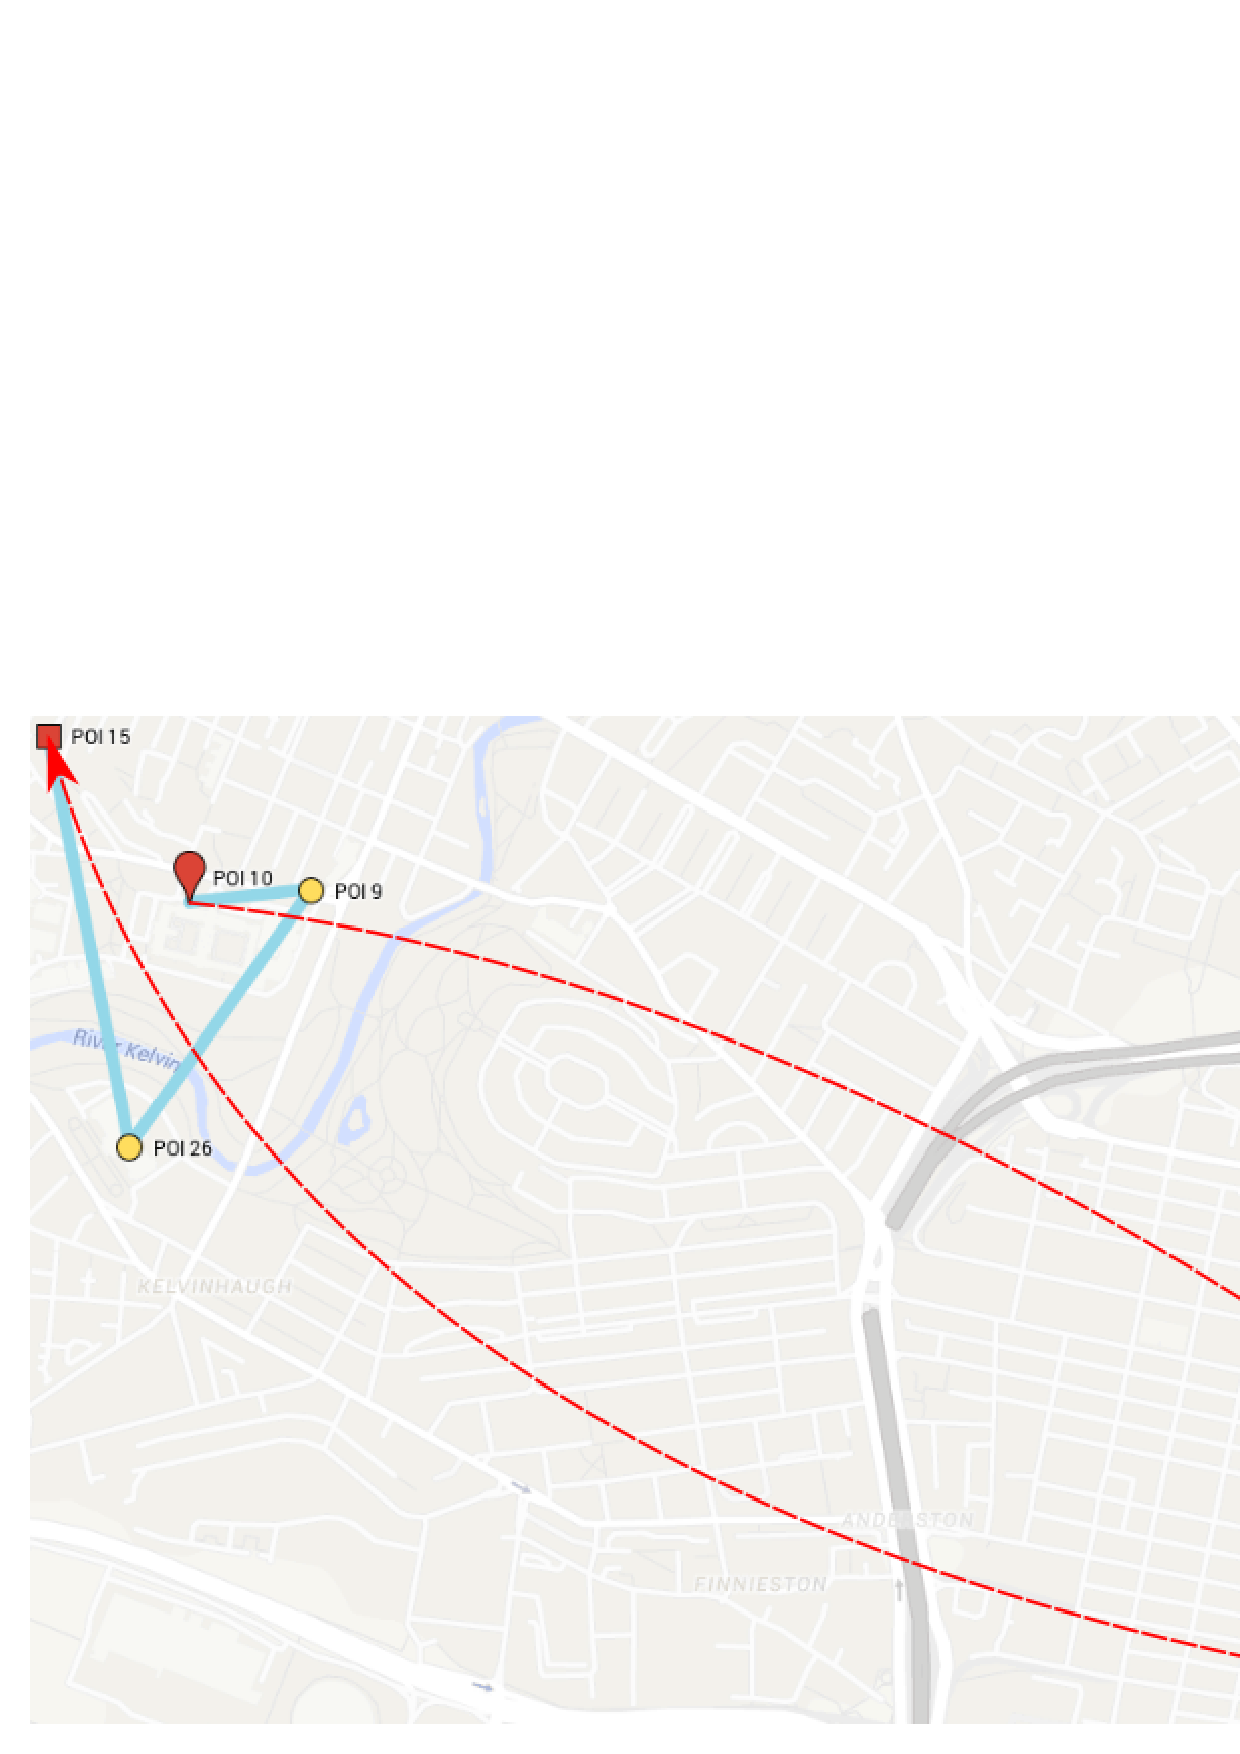
\includegraphics[width=\textwidth]{fig/poi_popularity.pdf}
\caption{Distribution of POI popularity}
\label{fig:popularity}
\end{figure*}

\begin{figure*}
\includegraphics[width=\textwidth]{fig/poi_nvisit.pdf}
\caption{Distribution of the number of visit at POI}
\label{fig:nvisit}
\end{figure*}

\begin{figure*}
\includegraphics[width=\textwidth]{fig/visit_duration.pdf}
\caption{Distribution of POI visit duration}
\label{fig:duration}
\end{figure*}

\begin{figure*}
\includegraphics[width=\textwidth]{fig/poi_transmat.pdf}
\caption{Transition matrices for $5$ individual POI features (Melbourne)}
\label{fig:transmat}
\end{figure*}


\section{POIs with same features}


By computing the Kronecker product of transition matrices of all the POI features,
we get an unnormalised transition matrix of POI features.
However, to obtain the transition probabilities between each POI pair $(p_i, p_j)$,
there are two cases needs to be dealt with properly:
\begin{enumerate}
\item POI features which represent POIs that do not exist in $\mathcal{P}$,
\item POI features that corresponds to more than one POIs in $\mathcal{P}$.
\end{enumerate}

% deal with feature vector without corresponding POI or with more than one POIs.
For the first case,
the corresponding rows and columns in the result matrix of Kronecker product are simply removed.

The second case was a bit subtle.
Let POIs with exactly the same features be a POI group,
the transition probabilities associated with POIs in the same group are computed as follows:
\begin{itemize}
\item The incoming (unnormalised) transition probability of the group was divided uniformly among POIs
      in the same group, which is equivalent to choose a POI in the group uniformly at random;
\item The outgoing (unnormalised) transition probability of each POI should be the same as the
      outgoing transition probability of the POI group, as one had already been in the POI group in this case;
\item The self-loop of the POI group represents the transitions between POIs in the same group,
      suppose the (unnormalised) transition probability from a POI group to itself is $P_o$,
      and the number of POIs in the group is $N_o$,
      the transition probability from $p_i$ to $p_j$ in the same group is
      \begin{displaymath}
          P(p_j | p_i) =
          \begin{cases}
              \hfill 0, \hfill & i = j \\
              \hfill \frac{P_o}{N_o - 1}, \hfill & i \ne j \\
          \end{cases}
      \end{displaymath}
\end{itemize}
Finally, the unnormalised outgoing transition probabilities of each POI were normalized to form
a valid probability distribution
\footnote{Note that dealing with the second case before or after the normalization leads to
the same transition probabilities, which can be easily proved. \cheng{Show proof}}.


\section{Experiment parameters}
% Parameters for IJCAI methods
The trade-off parameter for both \textsc{PersTour} and \textsc{PersTour-L} were $0.5$.
% Parameters for rankSVM
The regularization parameter of rankSVM was $10$ for all algorithms that utilising POI rankings, namely,
\textsc{PoiRank}, \textsc{Rank+Markov} and \textsc{Rank+MarkovPath}.
% Parameters for transition matrix
When computing the transition probabilities between POIs,
POI popularity, the total number of visit at POI and the average visit duration at POI were discritized using
$5$ bins uniformly in log-space, furthermore, POIs were grouped into $5$ clusters using K-means according to
their geographical locations.
% Parameters for Heuristics
The trade-off parameters $\alpha$ was set to $0.5$ in both \textsc{Rank+Markov} and \textsc{Rank+MarkovPath} algorithms.
% Parameters for SSVM
The regularization parameter to train \textsc{StructuredSVM} was $1$.


\section{Implementation details}
libsvmtools, PyStruct, Gurobi, etc.

There are about $12$\% of trajectories in Melbourne dataset that were failed to be evaluated
using \textsc{PersTour} due to the timeout of integer programming solver, the timeout is $2$ hours.
